\documentclass[12pt]{article}

\usepackage[utf8]{inputenc}
\usepackage{latexsym,amsfonts,amssymb,amsthm,amsmath}
\usepackage{graphicx}

\setlength{\parindent}{0in}
\setlength{\oddsidemargin}{0in}
\setlength{\textwidth}{6.5in}
\setlength{\textheight}{8.8in}
\setlength{\topmargin}{0in}
\setlength{\headheight}{18pt}



\title{ Sheet 2 }
\author{Our Names}

\begin{document}

\maketitle

\vspace{0.5in}



\subsection*{Exercise 1}
\begin{itemize}

\item[1.] 
\begin{itemize}
\item[(a)] \[
\mathcal{N}(\mu_{k},\Sigma_{k}) = \frac{1}{\sqrt{2\pi^{D} \det{\Sigma_k}}}e^{ -\frac{1}{2}(x-\mu_k)^\intercal \Sigma_k^{-1} (x-\mu_k)}
\]
\vspace{1cm} %Leave space for comments!
\[
g_k(x) = -\frac{1}{2} \log{\det{\Sigma_k}} - \frac{1}{2} (x-\mu_k)^\intercal \Sigma_k^{-1} (x-\mu_k) + \log \pi_k
\]
\vspace{1cm} %Leave space for comments!
\[
g_a(x) - g_b(x) \overset{!}{=} 0
\]
$$\longleftrightarrow\\$$
\[
-\frac{1}{2} \log{\det{\Sigma_A}} - \frac{1}{2} (x-\mu_A)^\intercal \Sigma_A^{-1} (x-\mu_A) + \log \pi_A
\]
\[ 
-\bigg( -\frac{1}{2} \log{\det{\Sigma_B}} - \frac{1}{2} (x-\mu_B)^\intercal \Sigma_B^{-1} (x-\mu_B) + \log \pi_B \bigg) = 0
\]
$$\longleftrightarrow\\$$
\[
\log{\det{\Sigma_B}}-\log{\det{\Sigma_A}}+(x-\mu_B)^\intercal\Sigma_B^{-1}(x-\mu_B)-(x-\mu_A)^\intercal\Sigma_A^{-1}(x-\mu_A)+2(\log{\pi_A}-\log{\pi_B})
\]
$$\longleftrightarrow\\$$
\[
x^\intercal\ \frac{1}{2} (\Sigma_A^{-1} - \Sigma_B^{-1})\ x + (\Sigma_A^{-1}\mu_A - \Sigma_B^{-1}\mu_B)\ x\ \]\[+\frac{1}{2} (\mu_B^\intercal \Sigma_B^{-1} \mu_B-\mu_A^\intercal \Sigma_A^{-1} \mu_A) + \log{{\pi_A}-\log{\pi_B}} + \frac{1}{2}(\log{\det\Sigma_B}-\log{\det\Sigma_A}) = 0
\]
\vspace{1cm} %Leave space for comments!
\[\Lambda = \frac{1}{2} (\Sigma_A^{-1} - \Sigma_B^{-1})\]
\[w = \Sigma_A^{-1}\mu_A - \Sigma_B^{-1}\mu_B\]
\[b = \frac{1}{2} (\mu_B^\intercal \Sigma_B^{-1} \mu_B-\mu_A^\intercal \Sigma_A^{-1} \mu_A) + (\log{\pi_A}-\log{\pi_B}) + \frac{1}{2}(\log{\det\Sigma_B}-\log{\det\Sigma_A})\]
A quadratic term indicates non linear decision boundry because quadratic equations are parabolic.
\vspace{1cm}
\item[(b)] 
\[
-\frac{1}{2} \log{\det{\Sigma}} - \frac{1}{2} (x-\mu_A)^\intercal \Sigma^{-1} (x-\mu_A) + \log \pi_A
\]
\[ 
+\frac{1}{2} \log{\det{\Sigma}} + \frac{1}{2} (x-\mu_B)^\intercal \Sigma^{-1} (x-\mu_B) - \log \pi_B = 0
\]
$$\longleftrightarrow\\$$
\[
 -(x-\mu_A)^\intercal \Sigma^{-1} (x-\mu_A) + 2\log \pi_A+(x-\mu_B)^\intercal \Sigma^{-1} (x-\mu_B) - 2\log \pi_B = 0
\]
\vspace{1cm}
\[
(x-\mu_k)^\intercal\Sigma^{-1}(x-\mu_k) = x^\intercal\Sigma^{-1}x-2\mu_k^\intercal\Sigma^{-1}x+\mu_k^\intercal\Sigma^{-1}\mu_k
\]
\vspace{1cm}
\[
 -(x-\mu_A)^\intercal \Sigma^{-1} (x-\mu_A)+(x-\mu_B)^\intercal \Sigma^{-1} (x-\mu_B) + 2(\log\pi_A - \log\pi_B) = 0
\]
$$\longleftrightarrow$$
\[
2(\mu_A-\mu_B)^\intercal\Sigma^{-1}x\ +\ (\mu_B^\intercal\Sigma^{-1}\mu_B - \mu_A^\intercal\Sigma^{-1}\mu_A)\ +\ 2(\log\pi_A -\log\pi_B) = 0
\]
$$\longleftrightarrow$$
\[
(\mu_A-\mu_B)^\intercal\Sigma^{-1}x\ +\ \frac{1}{2}(\mu_B^\intercal\Sigma^{-1}\mu_B - \mu_A^\intercal\Sigma^{-1}\mu_A)\ +\ \log\pi_A -\log\pi_B = 0
\]
\vspace{1cm}
\[w = (\mu_A-\mu_B)^\intercal\Sigma^{-1}\]
\[b = \frac{1}{2}(\mu_B^\intercal\Sigma^{-1}\mu_B - \mu_A^\intercal\Sigma^{-1}\mu_A)\ +\ \log\pi_A -\log\pi_B\]
\vspace{1cm} %Leave space for comments!
\end{itemize}
\item[2.] 
\begin{itemize}
\item[(a)] 
QDA decision boundary: \[
x^\intercal \begin{bmatrix}
\ 0.21008403 & -0.21008403 \\
-0.21008403 & \ 0.21008403
\end{bmatrix}x + \begin{bmatrix}
-1.53846154\\
-1.53846154
\end{bmatrix}x + 0.4436516
\]
\vspace{1cm}
LDA decision boundary: \[
\begin{bmatrix}
1.53846154\\
1.53846154
\end{bmatrix}x + 0
\]
\item[(b)]
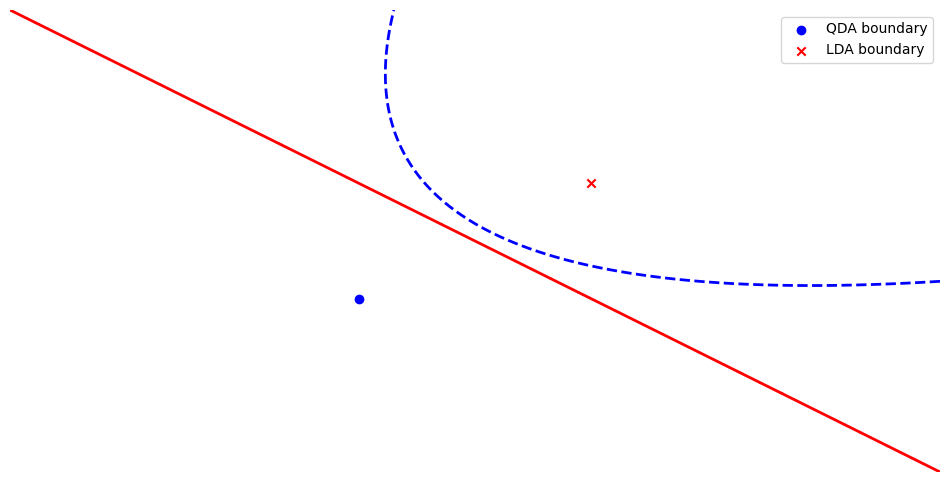
\includegraphics[scale=0.4]{image.png}
\item[(c)] 
The linear LDA boundary is preferred when the classes are of the same shape.
\vspace{1cm} %Leave space for comments!
\end{itemize}
\end{itemize}

\subsection*{Exercise 2}

\vspace{2in} %Leave more space for comments!







\end{document}
